% Options for packages loaded elsewhere
\PassOptionsToPackage{unicode}{hyperref}
\PassOptionsToPackage{hyphens}{url}
%
\documentclass[
  jou]{apa6}
\usepackage{lmodern}
\usepackage{amssymb,amsmath}
\usepackage{ifxetex,ifluatex}
\ifnum 0\ifxetex 1\fi\ifluatex 1\fi=0 % if pdftex
  \usepackage[T1]{fontenc}
  \usepackage[utf8]{inputenc}
  \usepackage{textcomp} % provide euro and other symbols
\else % if luatex or xetex
  \usepackage{unicode-math}
  \defaultfontfeatures{Scale=MatchLowercase}
  \defaultfontfeatures[\rmfamily]{Ligatures=TeX,Scale=1}
\fi
% Use upquote if available, for straight quotes in verbatim environments
\IfFileExists{upquote.sty}{\usepackage{upquote}}{}
\IfFileExists{microtype.sty}{% use microtype if available
  \usepackage[]{microtype}
  \UseMicrotypeSet[protrusion]{basicmath} % disable protrusion for tt fonts
}{}
\makeatletter
\@ifundefined{KOMAClassName}{% if non-KOMA class
  \IfFileExists{parskip.sty}{%
    \usepackage{parskip}
  }{% else
    \setlength{\parindent}{0pt}
    \setlength{\parskip}{6pt plus 2pt minus 1pt}}
}{% if KOMA class
  \KOMAoptions{parskip=half}}
\makeatother
\usepackage{xcolor}
\IfFileExists{xurl.sty}{\usepackage{xurl}}{} % add URL line breaks if available
\IfFileExists{bookmark.sty}{\usepackage{bookmark}}{\usepackage{hyperref}}
\hypersetup{
  pdftitle={Controlling the retrieval of general vs specific semantic knowledge in the instance theory of semantic memory},
  pdfauthor={Matthew Crump, Randall K. Jamieson, Brendan Johns, \& Michael Jones},
  pdfkeywords={keywords},
  hidelinks,
  pdfcreator={LaTeX via pandoc}}
\urlstyle{same} % disable monospaced font for URLs
\usepackage{graphicx}
\makeatletter
\def\maxwidth{\ifdim\Gin@nat@width>\linewidth\linewidth\else\Gin@nat@width\fi}
\def\maxheight{\ifdim\Gin@nat@height>\textheight\textheight\else\Gin@nat@height\fi}
\makeatother
% Scale images if necessary, so that they will not overflow the page
% margins by default, and it is still possible to overwrite the defaults
% using explicit options in \includegraphics[width, height, ...]{}
\setkeys{Gin}{width=\maxwidth,height=\maxheight,keepaspectratio}
% Set default figure placement to htbp
\makeatletter
\def\fps@figure{htbp}
\makeatother
\setlength{\emergencystretch}{3em} % prevent overfull lines
\providecommand{\tightlist}{%
  \setlength{\itemsep}{0pt}\setlength{\parskip}{0pt}}
\setcounter{secnumdepth}{-\maxdimen} % remove section numbering
\shorttitle{Negative information and expectation subtraction}
\affiliation{
\vspace{0.5cm}
\textsuperscript{1} Brooklyn College of CUNY\\\textsuperscript{2} Graduate Center of CUNY\\\textsuperscript{3} University of Manitoba\\\textsuperscript{4} McGill University\\\textsuperscript{5} Indiana University}
\keywords{keywords\newline\indent Word count: X}
\usepackage{csquotes}
\usepackage{upgreek}
\captionsetup{font=singlespacing,justification=justified}

\usepackage{longtable}
\usepackage{lscape}
\usepackage{multirow}
\usepackage{tabularx}
\usepackage[flushleft]{threeparttable}
\usepackage{threeparttablex}

\newenvironment{lltable}{\begin{landscape}\begin{center}\begin{ThreePartTable}}{\end{ThreePartTable}\end{center}\end{landscape}}

\makeatletter
\newcommand\LastLTentrywidth{1em}
\newlength\longtablewidth
\setlength{\longtablewidth}{1in}
\newcommand{\getlongtablewidth}{\begingroup \ifcsname LT@\roman{LT@tables}\endcsname \global\longtablewidth=0pt \renewcommand{\LT@entry}[2]{\global\advance\longtablewidth by ##2\relax\gdef\LastLTentrywidth{##2}}\@nameuse{LT@\roman{LT@tables}} \fi \endgroup}

\newlength{\cslhangindent}
\setlength{\cslhangindent}{1.5em}
\newenvironment{cslreferences}%
  {\setlength{\parindent}{0pt}%
  \everypar{\setlength{\hangindent}{\cslhangindent}}\ignorespaces}%
  {\par}

\title{Controlling the retrieval of general vs specific semantic knowledge in the instance theory of semantic memory}
\author{Matthew Crump\textsuperscript{1}, Randall K. Jamieson\textsuperscript{3}, Brendan Johns\textsuperscript{4}, \& Michael Jones\textsuperscript{4}}
\date{}

\authornote{Add complete departmental affiliations for each author here. Each new line herein must be indented, like this line.

Enter author note here.

Correspondence concerning this article should be addressed to Matthew Crump, 2900 Bedford Avenue, Brooklyn, NY. E-mail: \href{mailto:mcrump@brooklyn.cuny.edu}{\nolinkurl{mcrump@brooklyn.cuny.edu}}}

\abstract{
No abstract yet


}

\begin{document}
\maketitle

\hypertarget{introduction}{%
\section{Introduction}\label{introduction}}

Distributional models of semantics produce word embeddings sensitive to word co-occurrence structure in natural text corpora. Words appearing in similar local contexts (sentences, paragraphs) have more similar word embeddings than words appearing in different local contexts. The quality of word embeddings depends partly on their intended use. From an applied perspective, word-embeddings could be used to train a classifier (e.g., for sentiment analysis) and their quality assessed by classifier accuracy. From a basic perspective, distributional models have been forwarded as models of semantic knowledge and word-embedding quality is often measured by fits to human performance in semantic tasks. In both cases, word embedding quality depends on managing base rates of word occurence in natural text. For example, high frequency words that appear across contexts can easily dominate semantic vectors, causing all embeddings to become globally more similar and less indicative of nuanced meaning. Standard approaches to managing base rate information have questionable cognitive plausibility. The present work shows that a merger of assumptions between two instance-based memory models, the instance theory of semantics (ITS, Jamieson, Avery, Johns, and Jones (2018)) and the instance theory of associative learning (MINERA-AL, Jamieson, Crump, and Hannah (2012)), provides a cognitively plausible means of managing base rate information in the construction of word embeddings.

Distributional models employ various tactics to manage base rates of word occurence. The widespread practice of excluding high frequency stop words is a tacit recognition of base rate issues. Word-embeddings become less distinctive and meaningful when stop words are included because stop words co-occur frequently with all words. Stop word exclusion is often arbitrary and does not control for base rate influences from remaining words included in the corpus. Early models like LSA (Landauer \& Dutnais, 1997) dealt with base rates by transformation. For example, word frequencies were log transformed and divided by their entropy across document contexts. The log transform compresses frequency counts, and the division by entropy weights words by the specificity of their occurence in local contexts. As a result, high-frequency words ubiquitous across contexts (high entropy) are weighted less strongly than words peculiar to specific contexts (low entropy). More recent neural network models like word2vec (Mikolov, Sutskever, Chen, Corrado, \& Dean, 2013) deal with base rates by a process of subsampling adversial examples during training. For example, network weights are modified by prediction error from positive and negative examples. And, the negative examples are typically sampled randomly as function of their word frequency. Importantly, word2vec produces high-quality word embeddings that often explain more variance in human semantic judgments compared to other models (Mandera, Keuleers, \& Brysbaert, 2017), and these improvements have been attributed to the subsampling procedure.

Although we are optimistic that semantic cognition can be profitably understood in terms of distributional models, we question the cognitive plausibility of the above approaches to managing base rate information. For example, it is unlikely that people fail to encode stop words, it is unclear how they would weight word frequency knowledge by information theoretic transforms (or apply singular value decomposition), and we doubt that people routinely employ negative sub-sampling as they encounter words in everyday life. In our view, a satisfactory model should detail a cognitively plausible process for managing base rate of occurence information in constructing semantic knowledge. We propose a cognitive solution that merges insights form theoretical traditions in memory and learning.

Jamieson et al. (2018) applied instance-based memory theory to the problem of distributional semantics, combining BEAGLE-style word representations with MINERVA 2 encoding and retrieval operations to create ITS. ITS differs from standard distributional models in assuming instance-based representation rather than prototype representation. Semantic vectors in a standard BEAGLE model are memory-free prototypes. They are memory free because BEAGLE does not encode individual sentences, but instead compounds them into representations of individual words. They are prototypes because vectors are an aggregate sum over all of the sentence contexts in which particular words occur. These prototypical semantic vectors fail to capture polysemy. For example, ``bank'' could refer to a river or financial instution; but, a prototype representation glosses over the distinction and creates a single vector partway between the two meanings. By contrast, ITS assumes a role for memory to encode individual sentences as traces memory, and it produces semantic vectors for words at the time of retrieval. Retrieval is similarity driven and context-sensitive, allowing production of semantic vectors tailored to the local context (e.g., river vs.~piggy) of a probe word (e.g., bank).

Following standard practice, ITS used stop word exclusion to manage base rate information. Including stop words in BEAGLE style representations is highly problematic. For example, ITS used random vectors for each word, and represents sentences in memory by superposition of the word vectors in each sentence. Including stop words causes all sentences to become more similar to each other because they all routinely contain stop words. Consequently, retrieved semantic vectors become globally more similar and less sensitive to differences in word meaning. The purpose of this paper is to show that ITS can be modified to handle base rate information by including additional encoding and retrieval assumptions motivated by traditional learning theory. Briefly, instance-based processing assumptions from MINERVA 2 underpinning ITS have also been extended in MINERVA-AL to the problem of associative learning (Jamieson et al., 2012). MINERVA-AL accounted for numerous associative learning phenomena but used a discrepancy encoding rule, whereby only unexpected aspects of a novel experience were stored to memory. We show that a form of discrepancy encoding (termed weighted expectancy subtraction) can be applied in ITS to balance base rate information and provide control over the construction of more general or specific word meanings.

As an overview we first explain ITS and the proposed modifications. We are in preliminary stages of testing our approach, so we have elected to train ITS on an artificial language. The benefit of this approach is a clear accounting of how the original and modified versions of (ITS 2) respond to known co-occurence structure in the language. Following the model description and simulations we discuss how the assumptions of ITS 2 may be tested using a natural language corpus.

\hypertarget{its-and-its-2}{%
\section{ITS and ITS 2}\label{its-and-its-2}}

ITS 2 shares the same definition as its predecessor, except for the inclusion of weighted expectancy subtraction. If the weight is set to zero such that no expectancy is subtracted, then ITS 2 is identical to ITS. We first define ITS and then explain the ITS 2 modifications

\hypertarget{word-representation}{%
\subsection{Word representation}\label{word-representation}}

ITS combined representational assumptions from BEAGLE (Jones \& Mewhort, 2007) and processing assumptions from MINERVA 2 (Hintzman, 1986, 1984, 1988). From BEAGLE, words are treated as perceptual objects with no pre-existing semantic similarity. Each word is assigned an environment vector by randomly sampling \(n\) values from a normal distribution (\(\mu = 0\), \(\sigma = 1/n\)), where \(n\) determines the dimensionality of the vector space. As a result, all words are ortho-normal in expectation, and have an average of zero similarity to each other. ITS can accommodate other representational assumptions, and for clarity we adopt a simple identity matrix.

\hypertarget{memory}{%
\subsection{Memory}\label{memory}}

In ITS, slices of experience with words in context are represented as composite traces and stored as new row entries to a memory matrix. For example, committing a sentence to memory involves summing the environmental vectors for the words in the sentence:

\begin{equation}
M_i = c_i = \sum_{j=1}^{j=h} w_{ij}
\label{eq:memory}
\end{equation}

\(M_i\) is the memory matrix, and \(c_i\) is a sentence context. \(c_i\) is stored in a new row in \(M-I\) as a composite trace by summing the \(w_{ij}\) environment vectors for each word, from \(1\), to \(h\), in the sentence. For example, the sentence ``I like cats'' is the sum of \(w_{I} + w_{like} + w_{cats}\). The number of words inside a trace is a windowing parameter that must be larger than one word, otherwise the memory will return perceptually similar traces, rather than semantically similar ones.

\hypertarget{retrieval}{%
\subsection{Retrieval}\label{retrieval}}

Word meaning is constructed at the time of retrieval. ITS probes memory with a word, and returns an echo response. The echo response is taken as the semantic vector for the word. Words are compared for semantic similarity by comparing their respective echoes. Retrieval and echo construction follow MINERVA 2.

The echo is constructed in two steps. First, an environment vector for a word \(w_i\) serves as a probe to memory \(M\), and the cosine similarity between \(w_i\) and all traces \(M\) are computed to produce a vector of trace activations \(a_i\):

\begin{equation}
a_i = (\frac{\sum_{j=1}^{j=n}p_j \times M_{ij}}{\sqrt{\sum_{j=1}^{j=n}p_j^2}\sqrt{\sum_{j=1}^{j=n}M_{ij}^2}})^{tau}
\label{eq:activation}
\end{equation}

where, \(a_i\) is the activation (cosine similarity to probe) of trace \(i\) in memory, \(p_j\) are the \(jth\) features of the probe, \(M_{ij}\) are the \(jth\) features of each trace \(i\) in memory, and \(n\) is the number of columns in memory setting the dimensionality of the vector space. The vector of activations is raised to a power, \({tau}\), controlling a retrieval gradient.

The activation vector is record of similarity between the traces and the probe spanning the range \(-1\) to \(1\), with \(a_i = 1\) when a trace is identical to the probe, \(a_i = 0\) when a trace is orthogonal to the probe, and \(a_i = -1\) when the trace is opposite the probe.

In the second step, the activated traces are summed to produce a composite memory response, called the echo. Specifically, all traces in memory are multiplied by their activations, and the echo is formed by summing the weighted traces:

\begin{equation}
e_j = \sum_{i=1}^{i=m}\sum_{j=1}^{j=n}a_i \times M_{ij}
\label{eq:echo}
\end{equation}

where, \(e_j\) is the \(jth\) feature of the echo, \(m\) is the number of traces in memory, \(a_i\) is the activation of trace \(i\), and \(M_{ij}\) are the \(jth\) values of each trace \(i\) in memory. In ITS, the echo is used as the semantic representation for the probe word.

As a result, semantic similarity, \(r\), between two words is computed between their respective echoes using a cosine:

\begin{equation}
r(p_1,p_2) = \frac{\sum_{j=1}^{j=n}e_{1j} \times{} e_{2j}}{\sqrt{\sum_{j=1}^{j=n}e_{1j}^2}\sqrt{\sum_{j=1}^{j=n}e_{2j}^2}}
\label{eq:semanticsim}
\end{equation}

Origianlly, ITS fixed \(tau\) at a power of 3, and varying tau, say from 0 to 5, changes the retrieval gradient. The retrieval gradient selectivity in the composition of the echo. When \(tau\) is near zero, the retrieval gradient is a squashing square function and all activated traces are summed directly. When \(tau\) is 1, traces are weighted linearly by their similarities. When \(tau\) is greater than 1, traces are weighted by a power function of their similarities. In this case, echo content contains traces that are increasingly similar to the probe.

We now turn to modifications in ITS 2 that allow it to manage base rate information through a process of weighted expectancy subtraction. This process can be implemented in the model during encoding throughout training, or only at retrieval after training is complete. The encoding variant is more computationally expensive, as the contents of ITS 2 memory must be transformed over the course of training the model, on a trace by trace basis.

\hypertarget{its-2-weighted-expectancy-subtraction-at-encoding}{%
\subsection{ITS 2: weighted expectancy subtraction at encoding}\label{its-2-weighted-expectancy-subtraction-at-encoding}}

ITS 2 implements weighted expectancy subtraction during encoding in a similar manner to MINERVA-AL's discrepancy encoding rule. The difference is the subtraction between the probe and the echo is weighted by \(x\), controlling the amount of expectation to be subtracted. Weighted expectancy subtraction is applied at each step across training. For example, when a new sentence is experienced, the sentence context vector \(c_i\) is used as a probe to memory to generate an echo. The echo represents the memories expectation for the new sentence. If the new sentence is fully expected, then the memory can reconstruct the new sentence on the basis of its existing traces. The magnitude of the echo vector contains the sum of many traces, and is generally much larger than the magnitude of the sentence context vector. As a result, before subtraction, the probe and echo vectors are normalized,

\begin{equation}
c'_j = \frac{c_j}{\max | c_{j,n} |}
\label{eq:normprobe}
\end{equation}

where, \(c_j\) is a probe vector, and the elements of \(c_j\) are divided by the largest absolute value in \(c_j\), to produce the normalized \(c'_j\). Similarly, the echo is normalized such that,

\begin{equation}
e'_j = \frac{e_j}{\max | e_{j,n} |}
\label{eq:normecho}
\end{equation}

where, \(e_j\) is an echo vector, and the elements of \(e_j\) are divided by the largest absolute value in \(e_j\), to produce the normalized \(e'_j\).

Next, the new trace encoded to memory is defined by subtraction of a weighted normalized echo from the normalized probe,

\begin{equation}
M_{ij} = c'_j  - xe'_j
\label{eq:ITS2encoding}
\end{equation}

where, \(M_{ij}\) is the new row entry in the memory matrix, and \(x\) is a weighting parameter varying from 0 to 1, controlling how the extent which the normalized echo is subtracted from the normalized probe. When \(x\) is set to 0, ITS 2 becomes equivalent to ITS.

\hypertarget{its-2-weighted-expectancy-subtraction-at-retrieval}{%
\subsection{ITS 2: weighted expectancy subtraction at retrieval}\label{its-2-weighted-expectancy-subtraction-at-retrieval}}

ITS 2 can also conduct a similar operation of weighted expectancy subtraction at the time of retrieval. In this case, memory is constructed identically to ITS, except weighted expectancy subtraction occurs at retrieval through a two-step iterative retrieval process. A probe word generates an echo from memory, and the echo is submitted in an iterative retrieval step to generate a second echo. The semantic representation for the word is taken as a weighted subtraction of the normalized second echo from the normalized first echo.

The first echo \(e_1\) is generated in the usual way, but then resubmitted as a probe to construct \(e_2\) by the same equations \eqref{eq:activation} and \eqref{eq:echo} used to construct \(e_1\). Both \(e_1\) and \(e_2\) are normalized following equation \eqref{eq:normecho}. Whereas in ITS, the semantic representation for a word is defined as \(e_1\), the semantic representation for a word with weighted expectancy subtraction at retrieval in ITS 2 is:

\begin{equation}
s_i = e'_1 - xe'_2
\label{eq:ITS2retrieval}
\end{equation}

where, \(s_i\) is the semantic representation for the \(ith\) word, and \(x\) is a weighting parameter varying from 0 to 1 controlling the amount of \(e'_2\) subtracted from \(e'_1\). Again, when \(x\) is set to 0, ITS 2 becomes equivalent to ITS.

\hypertarget{simulations}{%
\section{Simulations}\label{simulations}}

\begin{figure*}

{\centering 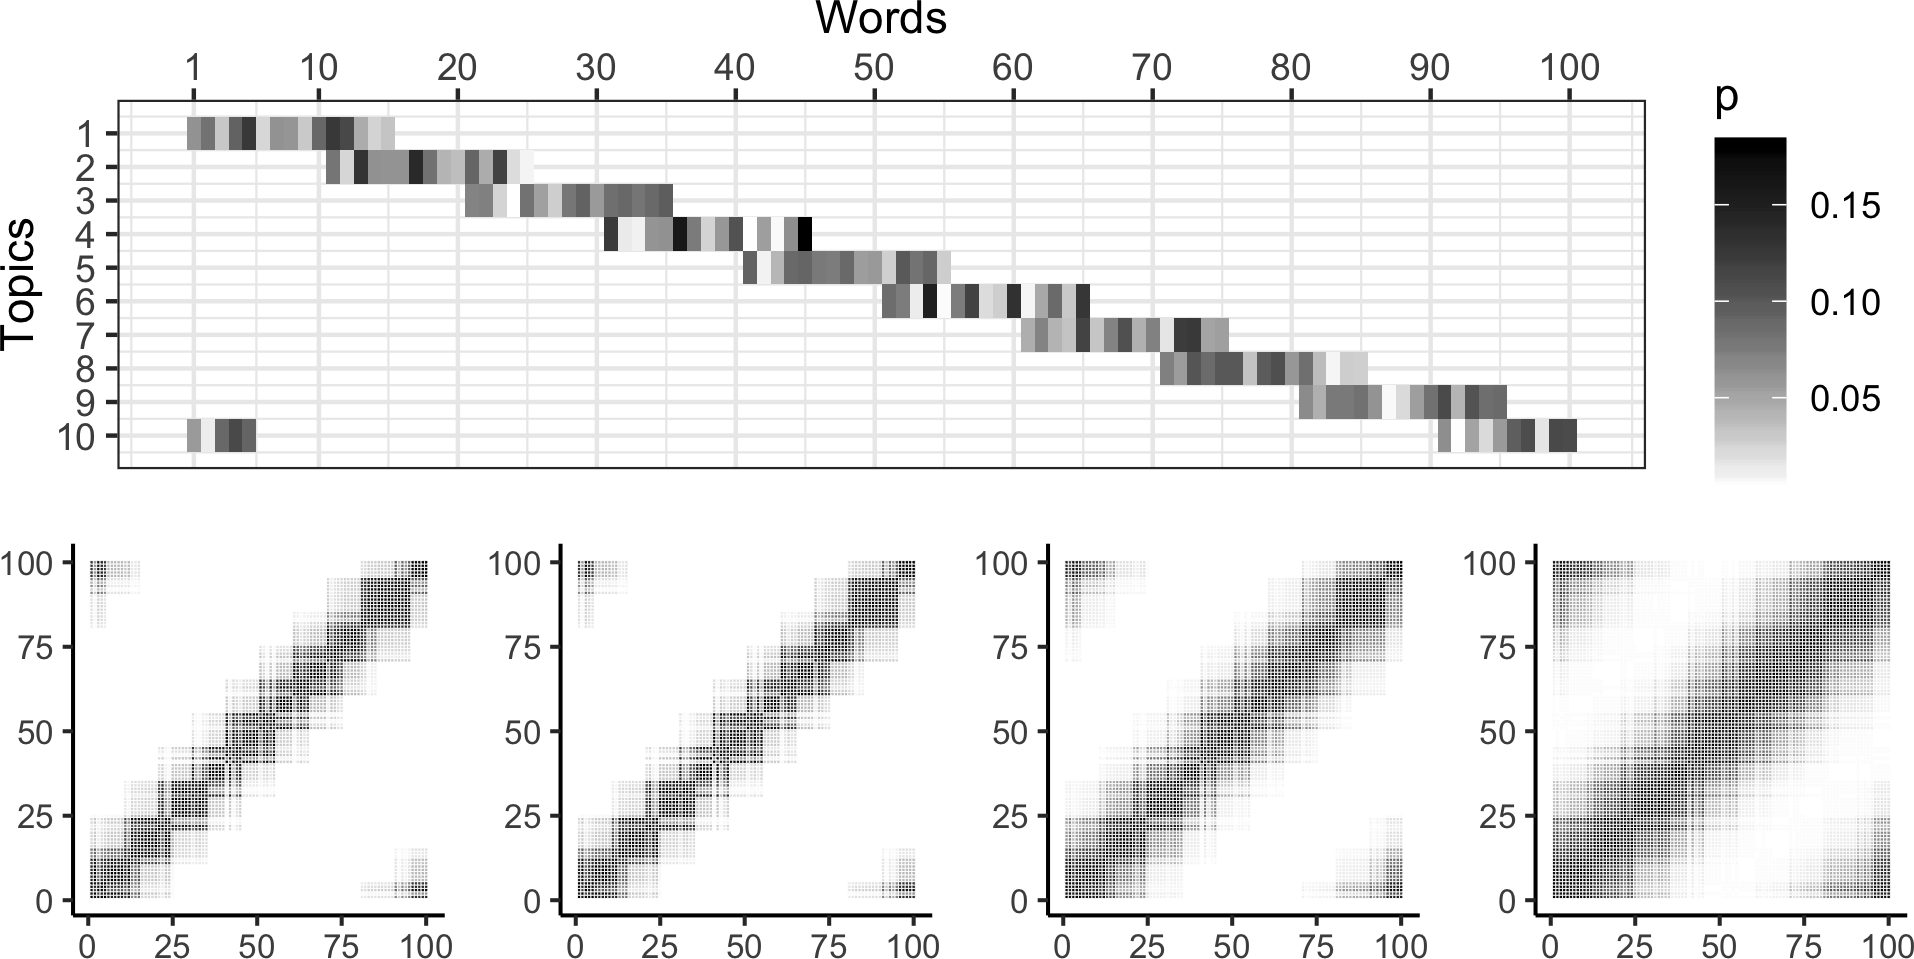
\includegraphics[width=\textwidth]{ITS_cogsci_files/figure-latex/artlang-1} 

}

\caption{A: The topic-word probability matrix defining the artificial language. Darker colors represent higher probability of word occurence. B1-4: Word-word similarity matrices from the first to fourth order.}\label{fig:artlang}
\end{figure*}

Our aim was to characterize how ITS and ITS 2 develop sensitivity to word co-occurence structure. First, we created an artificial language with known co-occurence structure. Next, we trained ITS on sentences from the artificial language and compared the semantic structure of ITS vectors to direct measures of the semantic structure of the language. Here, we were interested in determining which aspects of the language were recovered by ITS. Last, we determined whether the weighted expectancy subtraction process in ITS 2 would allow it to recover more veridical aspects of the co-occurence structure than ITS.

\hypertarget{artificial-language}{%
\subsection{Artificial language}\label{artificial-language}}

The artificial language contained no grammar, and only semantic structure based on word co-occurrence. The simplistic form offers a transparent window into the transformations of ITS 2. We assume that semantic topic generators use collections of words to discuss a given topic, and that word usage partially overlaps across topics. We define the language to contain 100 possible words, and 10 possible topics. Each topic uses 15 words, and overlaps by five words with the former and latter topics. Each topic had a random word-occurrence probability distribution that summed to one. Figure XA depicts the topic-word probability matrix defining the artificial language. A corpus is generated by randomly sampling a topic (equal probability), and then constructing a sentence from the topic by sampling \(n\) words as a function of their probability. Sentence-size varied randomly between 10 and 20 words per sentence. A corpus included 5,000 sentences.

The purpose of the simulations was to compare the semantic spaces generated by ITS and ITS 2 to known properties of the semantic space from the language. We defined the known semantic space at various orders of semantic similarity. At the first order, the true semantic representation for a word is the column vector for each word in the topic-word probability matrix above. To illustrate the semantic space we computed the cosine similarity between each word (using their column vectors) and plotted the similarity matrix. The word-word similarity matrix in figure \ref{fig:artwordsim1} shows the structure of the artificial language that models are ostensibly attempting to recover. Words are more similar to each other within their topics than between topics, and there is some overlap because word usage overlaps across the topics. Words in topic one are not at all similar to words in topic nine because there is no overlap in word usage between those topics. The remaining panels in figure \ref{fig:artwordsim1} show word-word similarity in higher order similarity space up to the fourth order. A higher order similarity space uses a lower-order space to derive a higher order one. For example, the second-order space uses columns from the first-order similarity matrix as word embeddings to compute a second word-word similarity space, and so on. In our language, because of word overlap between topics, words become increasingly similar to one another in higher order space. A veridical model would recover the first-order semantic space.

\hypertarget{simulation-1-simple-its}{%
\subsection{Simulation 1: Simple ITS}\label{simulation-1-simple-its}}

We trained a simplified version of the original ITS on 5000 sentences, using one-hot coding, or the identity matrix as environment vector for the words. Wach word was coded as a 1, with 99 zeroes. The position of the 1 in the vector refers to the \(nth\) word in the corpus. As a result, the memory matrix is equivalent to a document-term matrix of raw term frequencies occurring in each document. We used a range of retrieval gradients, setting tau between 0 and 9. We evaluated ITS at different training intervals, including memory for 100, 500, 1000, and 5000 sentences. At each interval we computed the echo as semantic representations for each word, and then a word-word similarity matrix from those vectors. To determine which aspects of the artificial language simple ITS recovered, we computed \(R^2\) between the ITS word-word similarity space, and the first to fourth order word-word similarity spaces derived directly from artificial language.

\begin{figure}
\centering
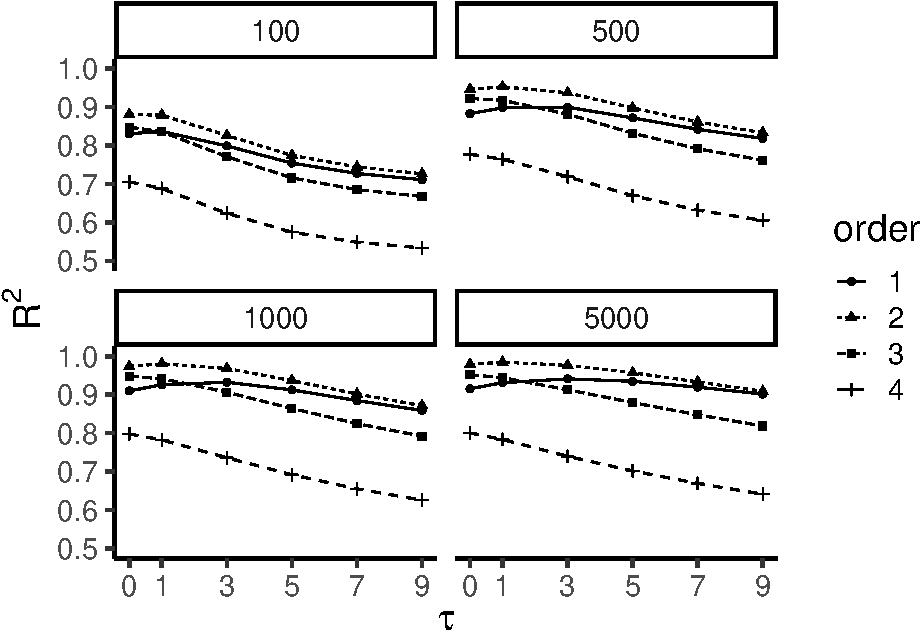
\includegraphics{ITS_cogsci_files/figure-latex/ITSsimple-1.pdf}
\caption{\label{fig:ITSsimple}\(R^2\) values between simple ITS word-word similarity space, and the first to fourth order word-word similarity spaces derived from the artificial language as a function of training, and retrieval gradient (tau)}
\end{figure}

Simple ITS performed very well in recovering the structure of artificial language. Most important, figure \ref{fig:ITSsimple} shows that simple ITS is most sensitive to the second-order similarity structure of the artificial language. More generally, ITS became more sensitive to the language over traingin, and less sensitive as tau increased. The fact that simple ITS prioritizes the second order over the first is its fatal flaw. The second order space is an overgeneralized version of the first, and blurs out the finer distinctions between word usage within the topic structures that generate the words. This is a base rate of word occurrence issue. Simple ITS recruits base rate word occurrence from across the topic generators. As a result, in the second order space, semantic vectors for words that overlap between topics take on an average meaning between the topics, rather than idiosyncratic meaning within each topic.

\hypertarget{simulation-2-its-2-encoding}{%
\subsection{Simulation 2: ITS 2 encoding}\label{simulation-2-its-2-encoding}}

In simulation 2 we train ITS 2 with weighted expectancy subtraction at encoding on the same artificial language. Critically, we show that weighted expectancy subtraction can cause ITS 2 to become more sensitive to first order word-word similarity than higher orders. In the simulations we vary the value of \(x\) (from .01 to .5) to subtract different amounts of the echo from the probe. The value of \(x\) causes systematic differences in ITS 2's sensitivity to higher order similarity structure. For clarity, we set \(tau\) to 1.

\begin{figure}
\centering
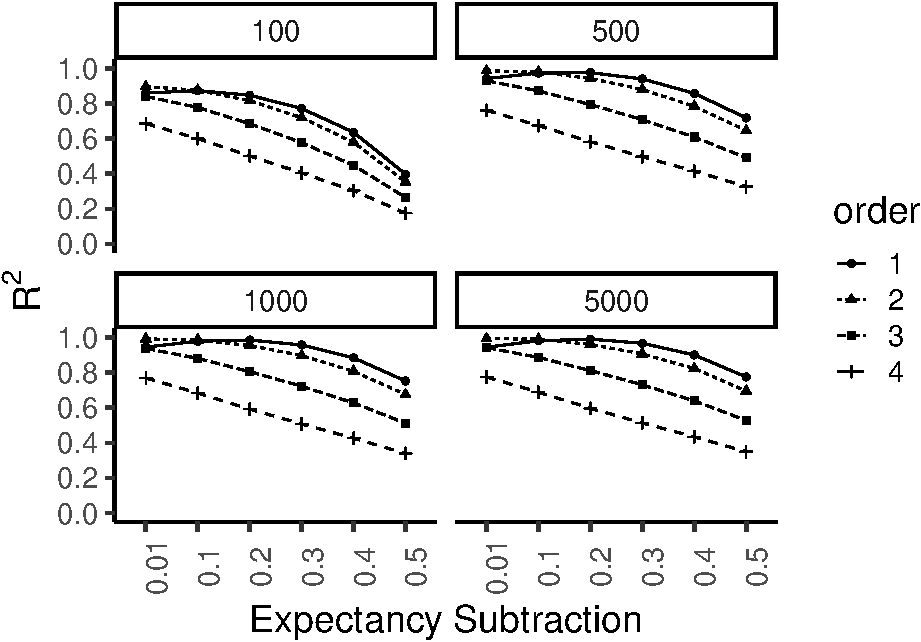
\includegraphics{ITS_cogsci_files/figure-latex/ITSencodinglinear-1.pdf}
\caption{\label{fig:ITSencodinglinear}\(R^2\) values between simple ITS word-word similarity space, and the first to fourth order word-word similarity spaces derived from the artificial language as a function of training, and weighted expectancy subtraction at encoding. The retrieval gradient (tau) was set to 1.}
\end{figure}

The effect of weighted expectancy subtraction at encoding is remarkable. First, ITS 2 recovered word-word similarity structure of the artificial language almost perfectly. Second, the amount of expectancy subtraction at encoding (\(x\)) modified the ordering of word-word similarity sensitivity. For example, when \(x=.01\), ITS 2 was most sensitive to second order word-word similarity, but become most sensitive to first-order word-word similarity as \(x\) increased. Finally, increasing \(x\) too much caused overall sensitivity to decline.

\hypertarget{simulation-3-its-2-retrieval}{%
\subsection{Simulation 3: ITS 2 retrieval}\label{simulation-3-its-2-retrieval}}

In simulation 3 we train ITS 2 with weighted expectancy subtraction at retrieval only on the same artificial language. We repeated the above simulation exactly, but used the equations involving one iterative retrieval step to conduct the weighted expectancy subtraction at retrieval. We also used a \(tau\) of 0 to compute both echoes, or a square retrieval gradient. We chose this value to foreshadow a clear correspondence between transformations of the defined artificial language in higher order similarity space, and what ITS 2 is achieving at retrieval by subtracting a portion of the second echo from the first.

\begin{figure}
\centering
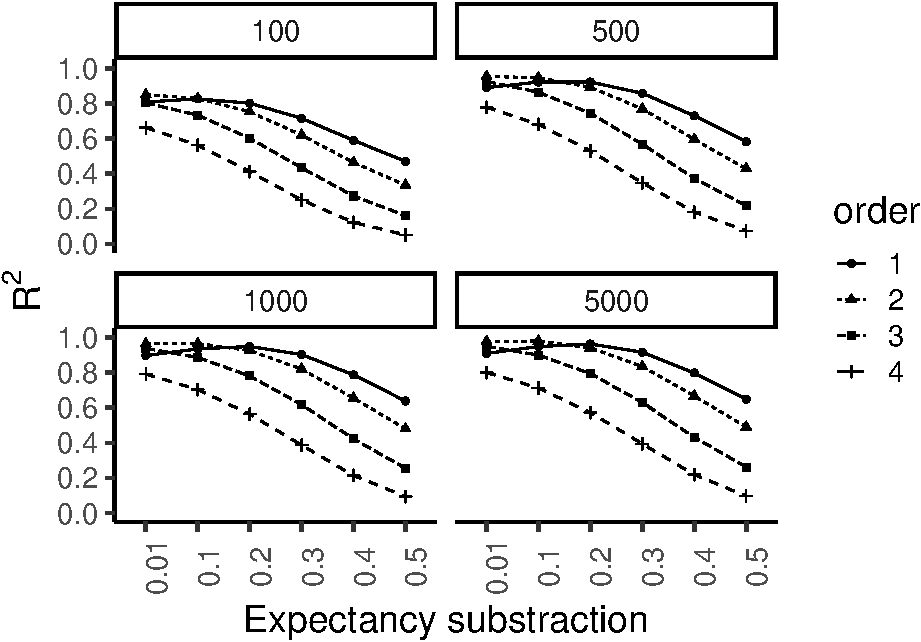
\includegraphics{ITS_cogsci_files/figure-latex/ITSretrieval-1.pdf}
\caption{\label{fig:ITSretrieval}\(R^2\) values between simple ITS word-word similarity space, and the first to fourth order word-word similarity spaces derived from the artificial language as a function of training, and weighted expectancy subtraction at retrieval.}
\end{figure}

The results of Simulation 3 are just as remarkable as the previous simulation. ITS 2 does not need to make any assumptions about encoding in order to benefit from weighted expectancy subtraction. The pattern of Simulation 3 is almost identical to that of Simulation 2. Specifically, ITS 2 does a good job of learning the word-word similarity structure, and it becomes most sensitive to first-order word-word similarity structure as \(x\) is increased. Again, increasing \(x\) has diminishing returns.

\begin{figure*}

{\centering 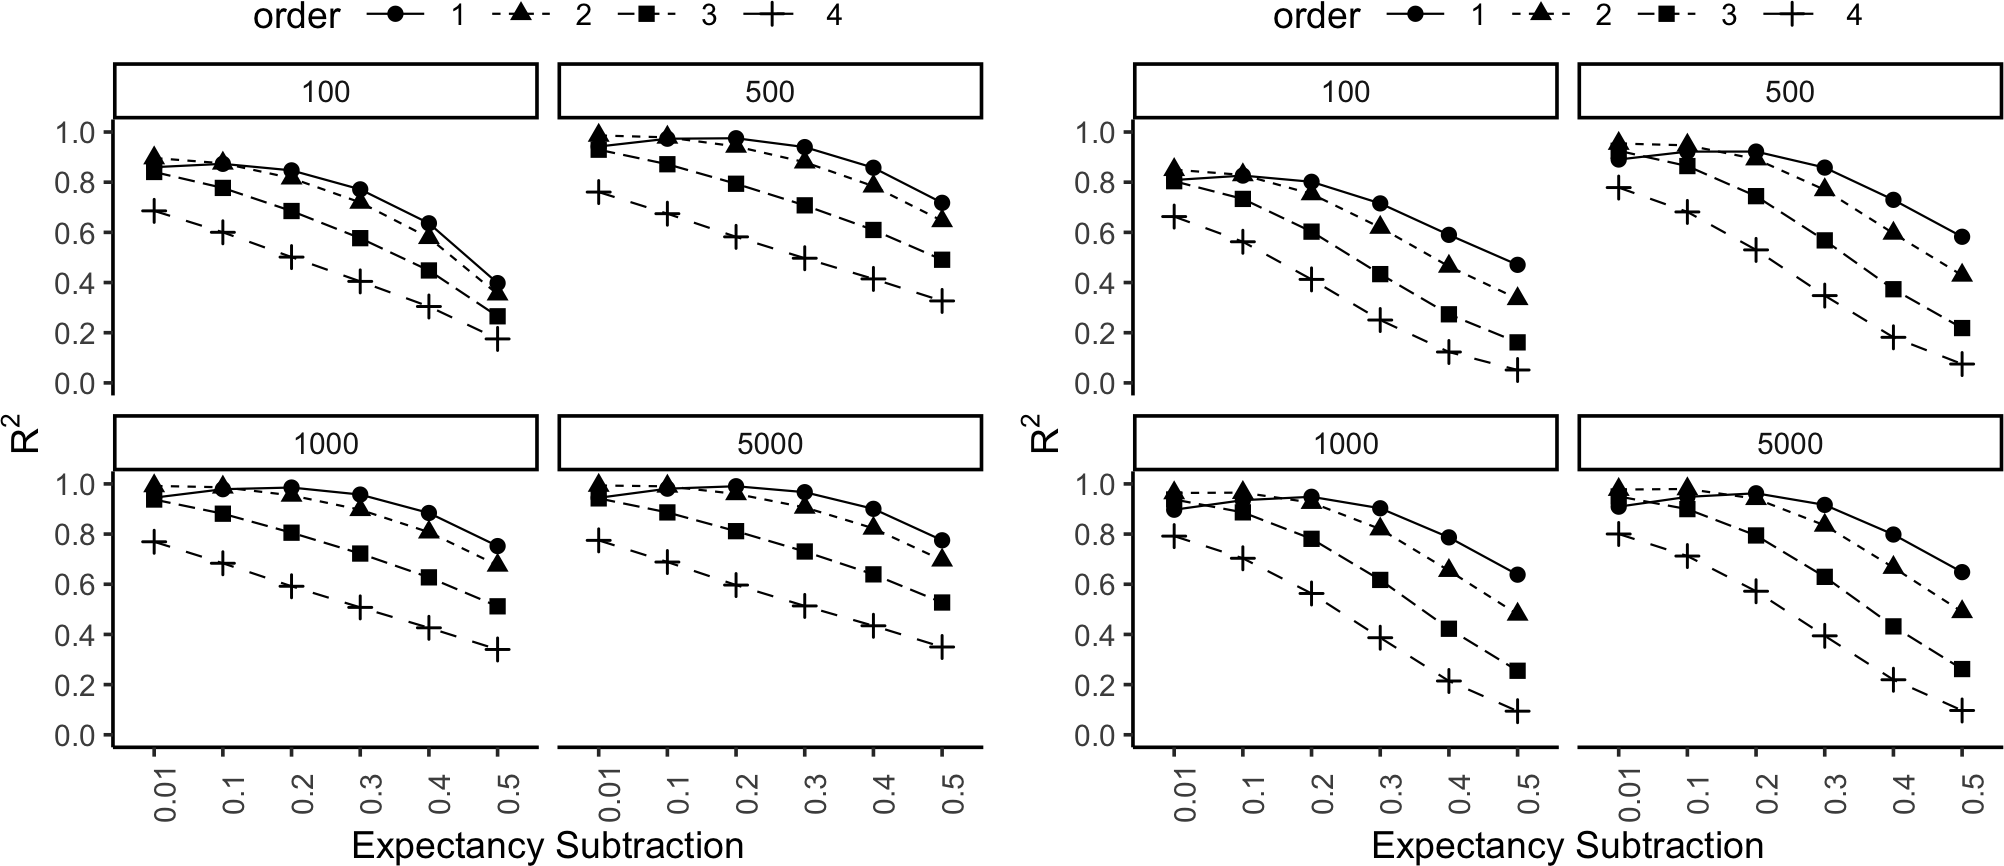
\includegraphics[width=\textwidth]{ITS_cogsci_files/figure-latex/allsims-1} 

}

\caption{blah blah blah}\label{fig:allsims}
\end{figure*}

\newpage

\hypertarget{references}{%
\section{References}\label{references}}

\begingroup
\setlength{\parindent}{-0.5in}
\setlength{\leftskip}{0.5in}

\hypertarget{refs}{}
\begin{cslreferences}
\leavevmode\hypertarget{ref-hintzmanSchemaAbstractionMultipletrace1986}{}%
Hintzman, D. (1986). Schema abstraction in a multiple-trace memory model. \emph{Psychological Review}, \emph{93}(4), 411--428.

\leavevmode\hypertarget{ref-hintzmanMINERVASimulationModel1984}{}%
Hintzman, D. L. (1984). MINERVA 2: A simulation model of human memory. \emph{Behavior Research Methods, Instruments, \& Computers}, \emph{16}(2), 96--101. doi:\href{https://doi.org/10.3758/BF03202365}{10.3758/BF03202365}

\leavevmode\hypertarget{ref-hintzmanJudgmentsFrequencyRecognition1988}{}%
Hintzman, D. L. (1988). Judgments of frequency and recognition memory in a multiple-trace memory model. \emph{Psychological Review}, \emph{95}(4), 528. Retrieved from \url{http://psycnet.apa.org/journals/rev/95/4/528/}

\leavevmode\hypertarget{ref-jamiesonInstanceTheorySemantic2018a}{}%
Jamieson, R. K., Avery, J. E., Johns, B. T., \& Jones, M. N. (2018). An instance theory of semantic memory. \emph{Computational Brain \& Behavior}, \emph{1}(2), 119--136. doi:\href{https://doi.org/10/gf6cm7}{10/gf6cm7}

\leavevmode\hypertarget{ref-jamiesonInstanceTheoryAssociative2012}{}%
Jamieson, R. K., Crump, M. J. C., \& Hannah, S. D. (2012). An instance theory of associative learning. \emph{Learning \& Behavior}, \emph{40}(1), 61--82. doi:\href{https://doi.org/10.3758/s13420-011-0046-2}{10.3758/s13420-011-0046-2}

\leavevmode\hypertarget{ref-jonesRepresentingWordMeaning2007}{}%
Jones, M. N., \& Mewhort, D. J. (2007). Representing word meaning and order information in a composite holographic lexicon. \emph{Psychological Review}, \emph{114}(1), 1. doi:\href{https://doi.org/10.1037/0033-295X.114.1.1}{10.1037/0033-295X.114.1.1}

\leavevmode\hypertarget{ref-landauerSolutionPlatoProblem1997}{}%
Landauer, T. K., \& Dutnais, S. T. (1997). A Solution to Plato's Problem: The Latent Semantic Analysis Theory of Acquisition, Induction, and Representation of Knowledge. \emph{Psychological Review}, \emph{104}, 211--240. doi:\href{https://doi.org/10/dcpw35}{10/dcpw35}

\leavevmode\hypertarget{ref-manderaExplainingHumanPerformance2017a}{}%
Mandera, P., Keuleers, E., \& Brysbaert, M. (2017). Explaining human performance in psycholinguistic tasks with models of semantic similarity based on prediction and counting: A review and empirical validation. \emph{Journal of Memory and Language}, \emph{92}, 57--78. doi:\href{https://doi.org/10/gfs3fg}{10/gfs3fg}

\leavevmode\hypertarget{ref-mikolovDistributedRepresentationsWords2013}{}%
Mikolov, T., Sutskever, I., Chen, K., Corrado, G. S., \& Dean, J. (2013). Distributed representations of words and phrases and their compositionality. In \emph{Advances in neural information processing systems} (pp. 3111--3119).
\end{cslreferences}

\endgroup

\end{document}
